% Generated by `uv run analyze`; needs \usepackage{pgfplots}
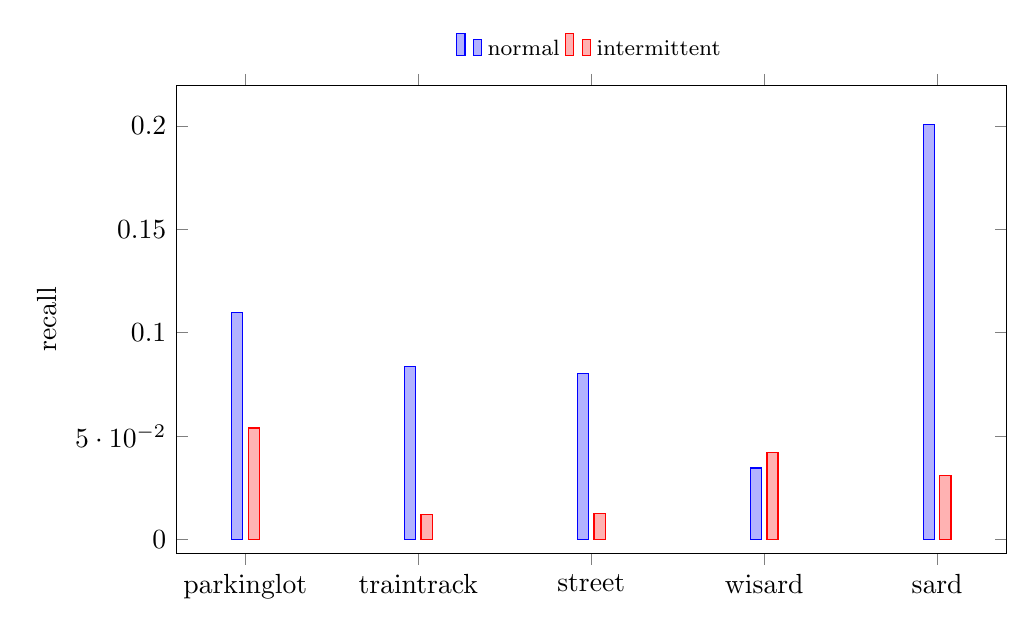
\begin{tikzpicture}
\begin{axis}[ybar, width=\columnwidth, height=0.62\columnwidth, bar width=4pt,
  symbolic x coords={parkinglot,traintrack,street,wisard,sard}, xtick=data, ylabel={recall},
  legend style={at={(0.5,1.03)}, anchor=south, legend columns=-1, draw=none, font=\footnotesize},
  error bars/y dir=both, error bars/y explicit]
\addplot coordinates {(parkinglot,0.1099) +- (0,0) (traintrack,0.08356) +- (0,0) (street,0.08043) +- (0,0) (wisard,0.03448) +- (0,0) (sard,0.2006) +- (0,0)};
\addlegendentry{normal}
\addplot coordinates {(parkinglot,0.05388) +- (0,0) (traintrack,0.01213) +- (0,0) (street,0.0126) +- (0,0) (wisard,0.04215) +- (0,0) (sard,0.03102) +- (0,0)};
\addlegendentry{intermittent}
\end{axis}
\end{tikzpicture}
